%; whizzy paragraph -pdf xpdf -latex ./whizzypdfptex.sh
%; whizzy-paragraph "^\\\\begin{frame}\\|\\\\emtext"
% latex beamer presentation.
% platex, latex-beamer でコンパイルすることを想定。 

%     Tokyo Debian Meeting resources
%     Copyright (C) 2012 Junichi Uekawa

%     This program is free software; you can redistribute it and/or modify
%     it under the terms of the GNU General Public License as published by
%     the Free Software Foundation; either version 2 of the License, or
%     (at your option) any later version.

%     This program is distributed in the hope that it will be useful,
%     but WITHOUT ANY WARRANTY; without even the implied warreanty of
%     MERCHANTABILITY or FITNESS FOR A PARTICULAR PURPOSE.  See the
%     GNU General Public License for more details.

%     You should have received a copy of the GNU General Public License
%     along with this program; if not, write to the Free Software
%     Foundation, Inc., 51 Franklin St, Fifth Floor, Boston, MA  02110-1301 USA

\documentclass[cjk,dvipdfmx,12pt]{beamer}
\usetheme{Tokyo}
\usepackage{monthlypresentation}

%  preview (shell-command (concat "evince " (replace-regexp-in-string "tex$" "pdf"(buffer-file-name)) "&")) 
%  presentation (shell-command (concat "xpdf -fullscreen " (replace-regexp-in-string "tex$" "pdf"(buffer-file-name)) "&"))
%  presentation (shell-command (concat "evince " (replace-regexp-in-string "tex$" "pdf"(buffer-file-name)) "&"))

%http://www.naney.org/diki/dk/hyperref.html
%日本語EUC系環境の時
\AtBeginDvi{\special{pdf:tounicode EUC-UCS2}}
%シフトJIS系環境の時
%\AtBeginDvi{\special{pdf:tounicode 90ms-RKSJ-UCS2}}

\newenvironment{commandlinesmall}%
{\VerbatimEnvironment
  \begin{Sbox}\begin{minipage}{1.0\hsize}\begin{fontsize}{8}{8} \begin{BVerbatim}}%
{\end{BVerbatim}\end{fontsize}\end{minipage}\end{Sbox}
  \setlength{\fboxsep}{8pt}
% start on a new paragraph

\vspace{6pt}% skip before
\fcolorbox{dancerdarkblue}{dancerlightblue}{\TheSbox}

\vspace{6pt}% skip after
}
%end of commandlinesmall

\title{東京エリアDebian勉強会}
\subtitle{第108回 2014年1月度}
\author{野島貴英}
\date{2014年1月18日}
\logo{
\includegraphics[width=8cm]{image200607/openlogo-light.eps}}

\begin{document}

\begin{frame}
\titlepage{}
\end{frame}

\begin{frame}{設営準備にご協力ください。}
会場設営よろしくおねがいします。
\end{frame}

\begin{frame}{Agenda}
 \begin{minipage}[t]{0.45\hsize}
  \begin{itemize}
   \item 注意事項
	 \begin{itemize}
	  \item 写真はセミナールーム内のみ可です。
          \item 出入りは自由でないので、もし外出したい方は、野島まで一声くださいませ。
	 \end{itemize}
   \item 最近あったDebian関連のイベント報告
	 \begin{itemize}
	  \item 第107回 東京エリアDebian勉強会
	 \end{itemize}
  \end{itemize}
 \end{minipage} 
 \begin{minipage}[t]{0.45\hsize}
  \begin{itemize}
   \item Debian Trivia Quiz
   \item Debian Pure Blend
  \end{itemize}
 \end{minipage}
\end{frame}

\section{イベント報告}
\emtext{イベント報告}

\begin{frame}{第107回 東京エリアDebian勉強会}

 東京エリアDebian勉強会107回目は(株)スクウェア・エニックスさんで開催されました。
5名の参加者がありました。

\begin{itemize}
\item 来年の勉強会の形式について参加者にてディスカッションをしました。\\
議論の内容:\url{http://debianmeeting.titanpad.com/debian2014?}
\item 野島さんが、Debian GNU/Hurd 2013について仮想環境による動作デモと、発表をしました。
\end{itemize}

 来年の勉強会の形式として、発表とハッカソン併用というのが有力な実施形式となりました。

 宴会は「世界のやまちゃん」にて行いました。


\end{frame}

\section{Debian Trivia Quiz}
\emtext{Debian Trivia Quiz}
\begin{frame}{Debian Trivia Quiz}

  Debian の常識、もちろん知ってますよね?
知らないなんて恥ずかしくて、知らないとは言えないあんなことやこんなこと、
みんなで確認してみましょう。

今回の出題範囲は\url{debian-devel-announce@lists.debian.org},
\url{debian-devel@lists.debian.org} に投稿された
内容などからです。

\end{frame}

\subsection{問題}
 %; whizzy-master ../debianmeetingresume201311.tex
% 以上の設定をしているため、このファイルで M-x whizzytex すると、whizzytexが利用できます。
%

\santaku
{PHPのメンテナチームを3つに分割する事が提案されました。分割されたグループの名前で間違っているのはどれ?}
{Debian PHP PECL Maintainers}
{Debian PHP PEAR Maintainers}
{Debian PHP DOCUMENT Maintainers}
{C}
{正しくは''Debian PHP Maintainers''です。以前、Debian PHP Maintainersは、PHP本体のパッケージも、PEARモジュールのパッケージも両方メンテナンスしていました。}

\santaku
{Debianについて、Debian Developer以外の人でも貢献したを讃えましょうということで、作られたサイトは?}
{advocates.debian.org}
{contributors.debian.org}
{superstar.debian.org}
{B}
{Debianに貢献したDebian Developer以外の人のアカウントが\url{http://contributors.debian.org/}にリストアップされるようになりました。なお、貢献についての集計の元は、\url{https://contributors.debian.org/sources/}に掲載されている情報を元に集計しているとの事です。}

\santaku
{2013/12後半頃にs390xアーキテクチャのデフォルトCコンパイラとしてのgccのバージョンが変更されました。どのバージョンになったのでしょう?}
{4.8}
{4.7}
{4.6}
{A}
{2013/12/23現在、powerpc/ia64/sparcアーキテクチャのデフォルトCコンパイラはまだgcc 4.6のようです。Debianの次期バージョンのJessieではgcc 4.6はサポート対象外なので早いところgcc 4.6から脱却する必要があります。}

\santaku
{2014/1に有名なデータベースがパッケージとして追加されました。何というデータベースでしょうか?}
{Maria DB}
{Percona DB}
{GDB}
{A}
{Maria DBは、LAMPシステムで有名なMysql DBの別の実装です。ついにMaria DBキター!今後のMysql依存のDebianのパッケージの動向が気になるこの頃です。}




\section{事前課題}
\emtext{事前課題}
{\footnotesize
 \begin{prework}{ 野島 貴英 }

 xmrisのパッケージ化の作業の続きをする。

\end{prework}

\begin{prework}{ 吉野(yy\_{}y\_{}ja\_{}jp) }

 (当日の東京エリアDebian勉強会で作業する内容を宣言してください という意味でしょうか)
\begin{itemize}
\item DDTSS
\item manpages-ja 続き
\end{itemize}

\end{prework}

\begin{prework}{ henrich }

fontチームのバグ潰しなど

\end{prework}

\begin{prework}{ dictoss(杉本 典充) }

FreeBSD portsのmpd5のdebパッケージ化を試みる

\end{prework}

\begin{prework}{ 野首 }

KAKASIのリリース作業を実施する。
debのnmu uploadも検討。

\end{prework}

\begin{prework}{ koedoyoshida }

最近サボっていたDDTSSでの翻訳作業を進める予定です。
\end{prework}


}



\section{Debian Pure Blend}
\emtext{Debian Pure Blend}

\begin{frame}{Debian Pure Blend}
 Debianに用意されている大量のパッケージをうまく使って、特定分野向けのシステムを容易にセットアップできるようにしたDebianの仕組み(考え方)となります。

 Debian Pure Blendのメタnパッケージに含まれるRecommends情報が利用されて、指定された特定用途のパッケージが導入される仕組みとなっています。
\end{frame}

\begin{frame}{Debian Pure Blend図示}
\begin{center}
\includegraphics[width=0.8\hsize]{image201401/debian-pure-blend.eps}
\end{center}
\end{frame}

\begin{frame}{用語}
\begin{itemize} 
\item Debian Pure Blend\\
そのままのDebianを用いて特定用途向けのDebianを実現\\
例: DebiChem, Debian Edu等
\item Debian Blend \\
一部のDebianでは未だ公式には採択されていないちょっとした変更を付け足し、残りはそのままのDebianを用いて特定用途向けのDebianを実現
\end{itemize}
\end{frame}

\begin{frame}{用語}
\begin{itemize} 
\item Debian Derivative \\
Debian派生物と日本語では言われる。目的は様々であり、Debianを元にした新しいディストリビューションを作るという点では共通。Debianをベースにしたかもしれないが、現在では大量の変更/新規機能を加えて作られているディストリビューション。\\
例:ubuntu, SteamOS
\item web sentinel\\
\url{http://blends.debian.org}。PureBlendの種類と搭載されているパッケージ及び開発状況を載せているページ。
\end{itemize}
\end{frame}

\begin{frame}{利用できるDebian Pure Blend}

 現在Debian unstableで見つかったPure Blend用のパッケージの一覧を載せます。
(パッケージ名中の''*''は、文字列を示します。)
\begin{itemize}
\item Debian Junior\\
子供向けのDebianを作る。パッケージ名:junior-* 
\item Debian Med\\
医療関係者向けのDebianを作る。\\
パッケージ名:med-* 
\item Debian Edu\\
学校の情報教育向けのDebianを作る。\\
パッケージ名: education-*,debian-edu-* 
\item Debian Science \\
科学技術向けのDebianを作る。\\
パッケージ名:science-* 
\end{itemize}

\end{frame}

\begin{frame}{利用できるDebian Pure Blend}

\begin{itemize}
\item Debian Multimedia \\
マルチメディア作成関係者向けのDebianを作る。\\
パッケージ名:multimedia-* 
\item DebianGIS \\
地理関係者向けのDebianを作る。\\
パッケージ名:gis-*
\item Debichem \\
化学関係者向けのDebianを作る。\\
パッケージ名: debichem-* 
\item Debian EzGo\\
中国語に対応したDebianの1つを作る。\\
パッケージ名:ezgo-* 
\end{itemize}

\end{frame}

\begin{frame}{利用できるDebian Pure Blend}

 なお、経緯を追いかけきれていないのですが、
\url{http://blends.debian.org/blends/ch04.html}
の''Existing Debian Pure Blends''に記載されている他のBlendのパッケージを自分は見つけることができませんでした。\\
\center{\Large だれか教えてー}
\end{frame}

\begin{frame}[containsverbatim]{使ってみる}

\begin{commandline}
$ sudo aptitude install junior-gnome
... junior-gnome/compris/gworldclock/mathwar
が導入される...
\end{commandline}
%$
\end{frame}

\begin{frame}[containsverbatim]{依存関係みる}

 試しに、先の例のjunior-gnomeの依存関係を調べてみます。

\begin{commandline}
$ apt-cache depends junior-gnome
  Depends: junior-tasks
  Depends: junior-config
  Recommends: gcompris
  Recommends: gworldclock
  Recommends: mathwar
\end{commandline}
%$
 
 Recommendsとして、gcompris/gworldclock/mathwarが指定されている事がわかります。

\end{frame}

\begin{frame}{Pure Blend用のパッケージを作ってみる}

設計:
\begin{itemize}
\item PJ名 \\
Debian-visualnovel 
(visualnovel用途向け) 
\item パッケージ名 
visualnovel-* 
\item tasksel用パッケージ 
visualnovel-task 
\end{itemize}
\end{frame}

\begin{frame}{Pure Blend用のパッケージを作ってみる}

 手順は勉強会資料を参照。\\
ダウンロードはこちら↓\\
\url{http://tokyodebian.alioth.debian.org/pdf/debianmeetingresume201401.pdf}

\end{frame}

\begin{frame}{おわりに}

 作るの簡単!ぜひ。

\end{frame}

\section{今後のイベント}
\emtext{今後のイベント}
\begin{frame}{今後のイベント}
\begin{itemize}
 \item 2014年2月 Debian勉強会。
 \item 2014年3月 OSC Tokyo/Spring 2014 東京エリアDebian勉強会出張。
\end{itemize}
\end{frame}

\section{今日の宴会場所}
\emtext{今日の宴会場所}
\begin{frame}{今日の宴会場所}
未定
\end{frame}

\end{document}

;;; Local Variables: ***
;;; outline-regexp: "\\([ 	]*\\\\\\(documentstyle\\|documentclass\\|emtext\\|section\\|begin{frame}\\)\\*?[ 	]*[[{]\\|[]+\\)" ***
;;; End: ***
